%%-*-latex-*-

\section{Methodology}

This proposal defines an interactive interface, called \vestige, which
is based on a \emph{tangible block\hyp{}world} with augmented reality
and \emph{software feedback} in order to ease the difficulties that
underlies learning recursion and functional programming.

%*******************************************************************************
\subsection{Concepts at Stake}
%*******************************************************************************

In functional programming, the most important data structure is the
\emph{list}. Lists, also called \emph{stacks}, are a data type where
the first element that enters in is the last to go out, that is, the
updates follow a ``Lust In, First Out'' (LIFO) rule. They have such an
important role that in some programming languages it is the main
native data structure found in the code. The more notorious of these
is \lisp, an old pioneer functional programming language born in 1958.
By representing even the programs as lists, \lisp programmers can
manipulate the source code as a data structure in order to expand the
domain of the language and its syntax.

In \vestige, a list is modeled as a stack of cubes. These cubes are
subjected to gravity, thus the stack is stable and forces the student
to only handle its topmost cube, as the algorithmic model mandates,
because manipulating another cube would lead the whole stack to
collapse.

Additionally, \vestige incorporates the use of technologies from the
field of Augmented Reality (AR), that is, a real time process that
creates the illusion of additional objects in a real life scene by
overlapping virtual objects on live video.

Finally, this application is not an interactive programming language
similar to those studied in the field of visual programming languages,
nor it is part of a development environment. Instead, the
application's main objective is \emph{transfer of training}, where it
is expected that students acquire problem solving abilities and
knowledge about writing \erlang code as a consequence of interacting
with the interface.

%*******************************************************************************
\subsection{Interaction}
%*******************************************************************************

\begin{figure}
  \begin{fminipage}
    \begin{description}
    \item[Item markers] represent atomic values. They can be placed on
      top of stacks, i.e., as elements, or on the table, where they
      denote a non\hyp{}stack value.
    \item[Stack markers] are markers that always remain at the bottom,
      where items are putted on top of. All stacks must have
      one of these markers. The empty stack is then represented by
      this marker alone. Generally, stacks are rarely moved due to the
      system's nature where the most common user\hyp{}interaction
      method is to exchange items among stacks.
    \item[Switch markers] are special blocks whose occultation by
      the student's hand triggers a snapshot defining the current the
      current scene. Only one can be present.
    \end{description}
  \end{fminipage}
  \caption{Types of markers}
  \label{fig:list:markers}
\end{figure}

The \vestige application challenges the student to solve a problem by
interacting with a scene constituted by stacks of cubes placed on a
board or a table. Physically, cubes are objects made out of paper,
wood, plastic, or virtually any workable material. Each cube is
identified by a \emph{marker}, that is, a tag stuck on one side, which
must face the camera. Markers are classified into three groups, as
seen in~\fig{fig:list:markers}. Their designs are particular to
\artoolkit (which is a back\hyp{}end for \osgart). Hence, markers are
the only physical difference among cubes.

\begin{figure}
  \centering
  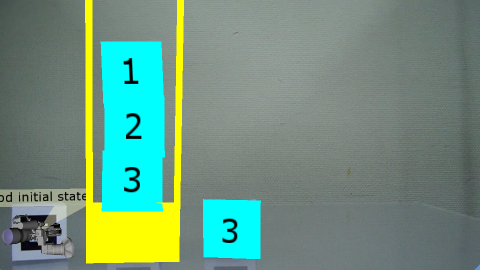
\includegraphics[width=0.45\textwidth]{img/iface/markers.png}
  \caption{The three types of markers}
  \label{fig:iface:markers}
\end{figure}

For each marker, an integer, a letter or a picture may be superimposed
to the video feed and sent to the display. More precisely, items are
described with a light blue square and a label that exhibits its
internal value. Stacks on the other hand are represented as a yellow
base with two sticks that grow accordingly to the number of blocks in
the stack. Finally, the switch is identified by a 3D\hyp{}model of a
camera as an abstraction of scenes and snapshots. These markers can be
easily recognized in~\fig{fig:iface:markers}. This 3D\hyp{}capable AR
feature is supported by another back\hyp{}end of \osgart, called \osg.

The stack data structure can be modified only by two simple
operations: \pop and \push. These operations are the minimum
required to build and change any stack. However, in \vestige it
is necessary to recognize the items' source and destination, including
a stack, the table (when it represents a value which is not a stack)
or outside the scene (when new items are created or discarded). As a
consequence, the resulting set of operations contains five basic
instructions as described in~\fig{fig:list:actions}.

\begin{figure}
  \begin{fminipage}{}
    \begin{description}
    \item[\pop:] moving the top block from a stack onto the table;
    \item[\push:] moving a block from the table onto the top of a
      stack (dual of \pop);
    \item[\poppush:] moving a top block from a stack on top of another
      stack (logical composition of \pop and \push);
    \item[\discard:] moving a block or stack out of the scene,
      regardless of where it is located;
    \item[\create:] moving a block or a stack from outside the scene
      onto the table or the top of a stack (dual of \discard).
    \end{description}
  \end{fminipage}
  \caption{User operations}
  \label{fig:list:actions}
\end{figure}

Altering a scene by different means or by combining at once two or
more of these operations is considered invalid. The only exceptions to
this rule are the \discard and \create operations, because the user
often creates or discards temporary data in the first and last steps;
dually, multiple cubes can be created or discarded in one single
operation. Any other situation is detected by the application, which
then stops the interaction with an error message explaining the cause
of the mistake. The blocks involved in the invalid move are augmented
with red and the system is stopped until the student restarts from
scratch by placing the blocks back into a valid initial scene. This
applies as well to logical mistakes, i.e., valid operations which are
recognized by the system as not conducing to the expected result,
other mistakes are said to be systemic.

A new scene is created each time an operation takes place, that is,
each time the user changes the position of one or more cubes. A
\emph{session} is a series of consecutive scenes and, as such, are
isomorphic to a run of the program, that is, a trace.
There are currently five types of sessions, also called
\emph{problems}, defined: reversing a stack, joining two stacks,
removing all the occurrences of a given block in a stack, removing all
consecutively repeated blocks and sorting by insertion a stack. In
order to control the user's actions, each problem can be executed in
two different modes: \emph{free} and \emph{supervised}. In the former
the student is allowed to freely, but validly, move the blocks. In
contrast, in the latter, each operation is checked to conform to a set
of \emph{step\hyp{}by\hyp{}step} rules which, as a whole, provide a
guided solution to the problem. When the operation does not match any
rule, the system considers it a logically invalid action, that is, the
blocks involved are augmented with red, a message explains the error
and prompts the student to restart the session.

During the whole interaction, the system communicates relevant
information to the user in three different manners: (1) by means of
messages, (2) by coloring blocks and (3) by displaying the actual
instance of the corresponding \erlang clause. Feedback messages' are
provided by a component in charge of drawing balloons above the cubes.
General messages are displayed in a balloon attached to the switch
marker, that is, the block with a camera icon projected, and
context\hyp{}specific messages can be displayed on each individual
marker. The coloring of blocks is a functionality integrated within
the markers logic where they are redrawn according to predefined
events. As mentioned previously, blocks augmented in yellow denote the
base of stacks and light blue blocks represent items belonging to a
stack. Yellow blocks will turn into red when an invalid movement takes
place. Finally, the system provides a feature that shows the actual
\erlang function call simulated by the interface. This reuses the
feedback subsystem by placing the code instantiation as a pop\hyp{}up
balloon over the switch cube.

Finally, a session ends with the system superimposing a congratulation
message when the student provides a correct (expected) and validly
obtained answer.

%*******************************************************************************
\subsection{Erlang}
%*******************************************************************************

From the point of view of didactics, the interface supports \erlang as
a target language. The pervasive use of lists in \erlang programs
makes them good candidates to be modeled by the block\hyp{}world
analogy. \erlang is a concurrent, functional programming language
originally created for prototyping and programming telecommunication
systems, like networks routers. Advanced programming language features
such as \emph{exceptions} or \emph{garbage collection} are part of
\erlang. Additionally, it is ideal for applications that require fault
tolerance, concurrency or distribution.

\renewcommand*\FancyVerbStartString{BEGIN-ADD}
\renewcommand*\FancyVerbStopString{END-ADD}
\begin{figure}[b]
  \fvset{frame=leftline,numbers=left,firstnumber=1,xleftmargin=3ex}
  \VerbatimInput{examples.erl}
  \caption{Add function}
  \label{fig:code:add}
\end{figure}

\renewcommand*\FancyVerbStartString{BEGIN-FIRSTG}
\renewcommand*\FancyVerbStopString{END-FIRSTG}
\begin{figure}[b]
  \fvset{frame=leftline,numbers=left,firstnumber=1,xleftmargin=3ex}
  \VerbatimInput{examples.erl}
  \caption{FirstG function (First element greater than N)}
  \label{fig:code:firstg}
\end{figure}

A program in \erlang consists of a set of functions logically bundled
in modules. A function is a series of \emph{clauses}, each
corresponding to a specific configuration of the input, that is, the
arguments. This is how many functions are defined in mathematics, like
the functions \texttt{add} shown by~\fig{fig:code:add} and
\texttt{firstg} shown by~\fig{fig:code:firstg}. The first function
adds a value into a list only when it is not already contained and the
second function finds the first element in a list that is greater than
a given value.

A clause is made of a \emph{pattern}, describing a specific input and
an \emph{expression} which is the result value of the function. The
pattern and the expression are separated by an arrow
(\verb|->|). This means that when the function's input
matches a pattern, the associated expression is evaluated in turn and
its value becomes the output of the function. In the first line of
code in~\fig{fig:code:add}, \texttt{f(I,[])} is the pattern and
\texttt{[I]} is the expression.

Patterns start with the function name followed by the input parameters
which are inside the parenthesis symbols ``\texttt{(}'' and
``\texttt{)}'' and are separated by the symbol comma
``\texttt{,}''. As a consequence,
line 1 of~\fig{fig:code:add} defines a function called \texttt{add}
with two input parameters \texttt{I} and \texttt{[]}. Input
parameters can be assigned to variables by using a string with an
uppercase first character as denoted by \texttt{I} in the first line
of~\fig{fig:code:add}. If the special symbol ``\texttt{\_}'' is used the
parameter is only matched but not assigned to any variable, this can
be seen in line 2 of~\fig{fig:code:firstg}. Lists can be defined with
the symbols \texttt{[} and \texttt{]}. Additionally, the symbol
\textbar inside a list denotes the separation between the
\emph{header} and the \emph{rest}. Therefore, an empty list, as the
one in the first pattern of~\fig{fig:code:add}, is stated as
\texttt{[]}, while a non\hyp{}empty list, as the one in the third
pattern can be stated as \texttt{[J|L]} where \texttt{J} is the
header and \texttt{L} is the rest. Additionally to simple pattern
rules, conditions can also be declared within the pattern by using the
special word \texttt{when}. One condition is present in the first
pattern the code in~\fig{fig:code:firstg}. Here, in order to match
the pattern, \texttt{I}, the header of the list of the first input
parameter, must be greater than \texttt{N}, the second input
parameter. Finally, patterns are matched top\hyp{}down, this means
that when the input fails to match the first clause then the system
will attempt the second, then the third and so on.

Expressions can be either a value or a function call. In the
interface values are usually variable that contains the result after
being processed by previous recursive calls. Function calls are
represented by the function's name followed by parenthesis that
embrace the input parameters which are separated by commas. Finally,
\erlang function clauses are separated by the semicolon symbol
``\texttt{;}'' except for the last clause of the function which
instead is marked by the dot ``\texttt{.}'' symbol.

\begin{figure}
  \centering
  \subfigure[Previous state]{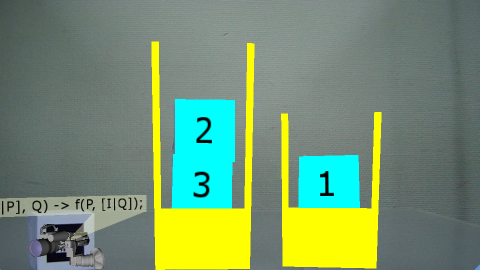
\includegraphics[width=0.45\textwidth]{img/iface/prevstate.png}}
  \subfigure[Next state]{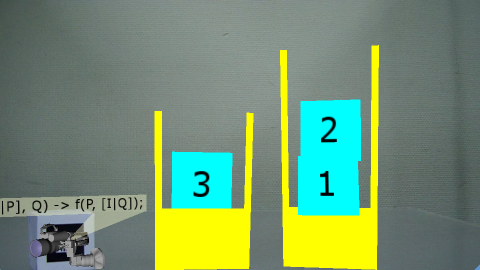
\includegraphics[width=0.45\textwidth]{img/iface/nextstate.png}}
  \caption{\texttt{f([2,3]) -> f([3],[2,1])}}
  \label{fig:iface:states}
\end{figure}

In the end, the main reason to choose \erlang for teaching, among
other functional languages, is its minimalist syntax and pattern
matching feature. The latter is used to easily assign and define
variables to parts of the input and to separate different cases. This
allows static overloading which means that a function can be defined
several times for different types of input parameters. Consequently,
programs syntax can be seen as the combination of the pattern matching
side and the clauses side. \vestige simulates this behavior with the
use of \emph{states} as flow mechanism. Here, the \emph{previous state}
is analog to the \emph{pattern} and the \emph{next state} is analog to
the \emph{expression}. A visual representation of this process can be
seen on~\fig{fig:iface:states}, here, a recursive call of an example
function \texttt{f} is set by altering the input parameters by means
of a \poppush operation.

%*******************************************************************************
\subsection{Didactic Phases}
%*******************************************************************************

The didactic process is made up of three phases. An initial phase
works to get the student acquainted with fully concrete instances of
some algorithmic problems, the second phase introduces the student to
the process of \emph{generalization}, the third phase aims at giving
rise to \emph{abstraction}, and finally, the student will hopefully be
ready to \emph{write} \erlang code after the third phase.

The first phase is composed of \emph{concrete scenarios}. The student
is asked to arrange stacks of blocks with superimposed random small
integers with the objective of solving one given problem. This can be
done by choosing either \emph{free} or \emph{supervised execution
  modes}, according to the student's skill. This phase can be run
several times if the student shows no progress.

The second phase introduces the student to \emph{generalizations} and
it also provides him with a deeper understanding of stacks. In this
phase, \emph{information hiding} is introduced, more precisely, only
numbers at the top of the stacks are displayed. As a consequence,
student's actions will be focused on the smallest part of the data
which is needed to make his way towards the result. For instance, each
time a \poppush operation is performed, only the topmost blocks are
shown. This will help the student to identify general cases and not
rely on \emph{global knowledge}.

In the third phase, \emph{variables} are superimposed on the items
blocks instead of random integers. Again, several instances of the
same problems are proposed. This phase prepares the student to the
transfer to textual programming by putting together the concepts of
generalization of cases and variables.

After the final phase, the student is expected not to rely on the
interface and instead he directly programs the \erlang functions
corresponding to the problems solved in the previous phases. To
achieve this, the student is provided with a further explanation on
how to symbolically translate the actions with the interface into
\erlang code.

%*******************************************************************************
\subsection{System Internals}
%*******************************************************************************

Scenes are captured as a whole by a camera in order to be processed as
the main input to a visual recognition subsystem. This subsystem
generates a logical representation of the scene according to the
physical location of the cubes and their relative position with each
other. Hence, the system is constituted by two views: a physical view
that consists of physical markers and a logic view that abstracts
them. Internally the physical view is composed by \texttt{markers} and
supported by a always running process in charge of augmenting them on
the screen. On the other hand, the logical view is composed by
\texttt{nodes} and it is supported by the \vestige's
\emph{main process} which is triggered when the student hides the
\emph{switch} marker.

The main process is handled by a component called \texttt{Step}. This
component itself is branched in two different sub\hyp{}processes. One
called \emph{initial sub\hyp{}process} to approve a valid
\emph{initial state} and define a set of \texttt{Rules}. The other is
called \emph{repetitive sub\hyp{}process} and its main objective is to
treat the subsequent states and validate the \emph{final state}.

\begin{figure}[!h]
  \centering
  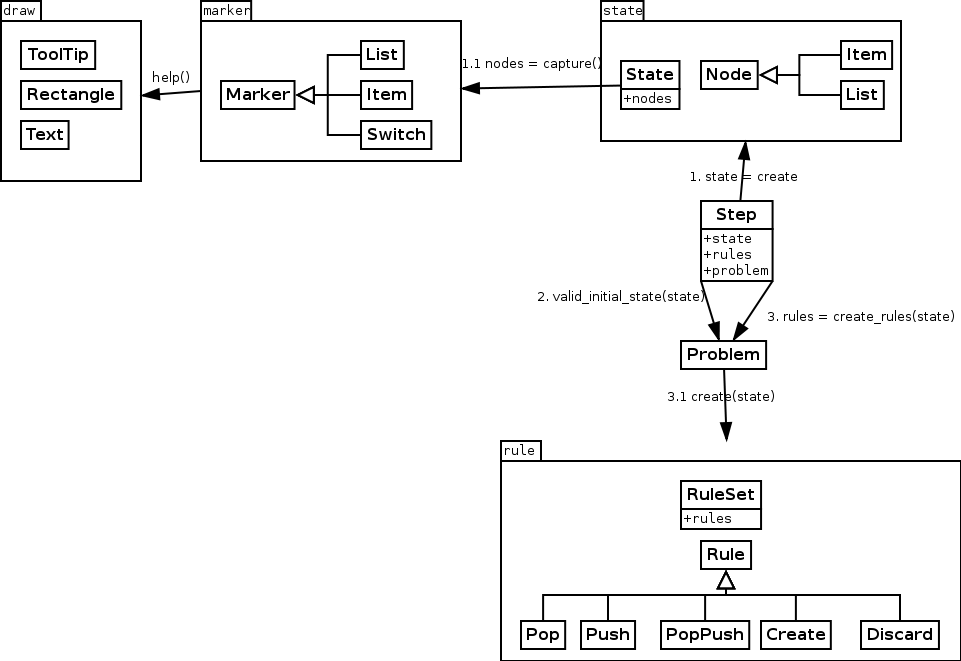
\includegraphics[width=0.8\textwidth]{img/diagrams/initial.png}
  \caption{Initial Sub\hyp{}process Diagram}
  \label{fig:dia:initial}
\end{figure}

The \emph{initial sub\hyp{}process} is described
in~\fig{fig:dia:initial}. It starts by capturing the current state of
the markers according to their relative position to the camera. A
state is nothing but a \emph{tree} with two \emph{levels of depth}.
The first level is composed by either \emph{list nodes} (a conceptual
representation of a list marker) or \emph{item nodes} (a conceptual
representation of an item marker) and the second level is composed
exclusively by item nodes which are children of first\hyp{}level
lists. This tree is generated by comparing blocks' positions in order
to identify item markers aligned with list markers. States only
contains the data acquired from the physical world and for this reason
they are the main source of information used by the application.

After the \emph{initial state} is captured, the control is given to
the \texttt{Problem} component. This component is where student
exercises are defined. It is in charge of validate \emph{initial} and
\emph{final scenes} and dynamically creating \emph{positive
  scenarios}, that is, admissible execution traces for different
possible \erlang functions corresponding to the exercise. In \vestige,
five different problems are implemented: \emph{Reverse}, \emph{Join},
\emph{Remove All}, \emph{Compress} and \emph{Insertion Sort}. However,
because of the simplicity of the \texttt{Problem} mechanism, the
application could be easily expanded.

Each session has only one current \texttt{Problem}. Thus, the way to
validate the initial state varies because different exercises expect
different input. Positive scenarios are also generated according to
the \texttt{Problem}. Internally, they are called \texttt{Rules},
which are a more generic view of \texttt{actions}. \texttt{Rules} are
used only during \emph{supervised} execution mode in order to warrant
that the user will provide a valid final solution. There are four
types of \texttt{Rules}: \pop, \push, \poppush, \create and \discard.
Each one validates if its dual \texttt{action} as described
in~\fig{fig:list:actions} is executed when expected. After this, the
control is returned to the \texttt{Step} component.

\begin{figure}[t]
  \centering
  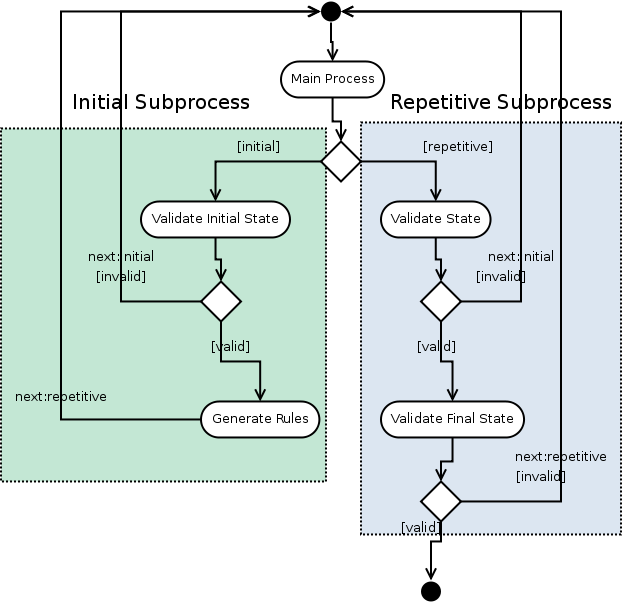
\includegraphics[width=0.6\textwidth]{img/diagrams/main.png}
  \caption{Main Process Diagram}
  \label{fig:dia:main}
\end{figure}

The \emph{initial sub\hyp{}process} will be executed again until a
valid \emph{initial state} is verified and \texttt{Rules} are
correctly generated. Once this is done, the \emph{main process}
switches to iterations of the \emph{repetitive sub\hyp{}process}, this
can be seen in~\fig{fig:dia:main}.

\begin{figure}[!b]
  \centering
  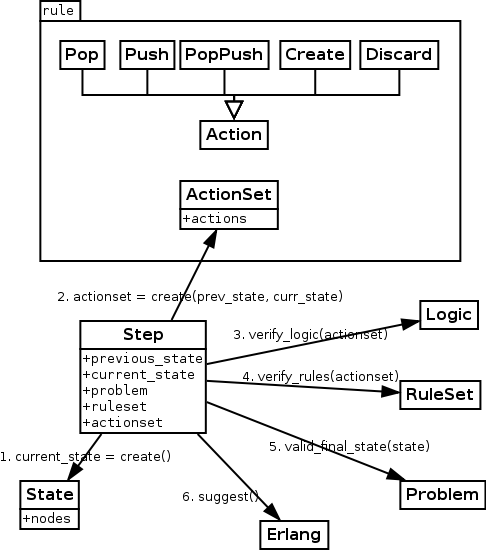
\includegraphics[width=0.5\textwidth]{img/diagrams/repetitive.png}
  \caption{Repetitive Sub\hyp{}process Diagram}
  \label{fig:dia:repetitive}
\end{figure}

The \emph{repetitive sub\hyp{}process}, in
the~\fig{fig:dia:repetitive}, starts by capturing the \emph{current
  state}. It then identifies the \texttt{actions} executed by the user
by comparing the \emph{current} and \emph{previous states}. In optimal
conditions, this difference would consist of a single \texttt{action}
as shown by~\fig{fig:list:actions}. Additionally, a special type is
defined to identify invalid user movements such as performing \pop on
an item which is not at the top of a list or executing multiple
actions at once. \create and \discard are an exception of this rule
because two or more items can be created or discarded in a single
step. After detecting \texttt{logic actions}, and when in
\emph{supervised mode}, the system validates that the user has moved
the blocks as expected according to the \texttt{Rules} component. If
the \texttt{action} is invalid by either \emph{logic} or \emph{rules},
the system asks the student to restart the interaction from a valid
initial state. Finally, if the current state is a valid final state
the system finishes the interaction by presenting a congratulations
message. Otherwise, \erlang code suggestions are displayed. The
repetitive sub\hyp{}process is executed cyclically until the latter
condition is fulfilled.

Finally, the \texttt{core} component is formed by two modules in
charge of low\hyp{}level operations and of interfacing external
libraries. The first module is the \texttt{drawing helpers} which
defines the necessary mechanisms to augment 3D objects over the input
video; this is an interface to the \osg module of \osgart. The second
module is called \texttt{global data} and it is in charge of store
general information such as the application parameters and \osgart
basic objects. This component is of vital importance because it
supports the whole system.
